\documentclass[portrait,a0paper,fontscale=0.28]{baposter} % Adjust the font scale/size here

\usepackage{graphicx} % Required for including images
\graphicspath{{figures/}} % Directory in which figures are stored

\usepackage{amsmath} % For typesetting math
\usepackage{amssymb} % Adds new symbols to be used in math mode


%\usepackage{subfigure,float}
%\usepackage{subfig}
%\usepackage{subfloat}
%\usepackage{subcaption}
%\usepackage{float}
\usepackage{pgf}
%\usepackage{minipage}
\usepackage{tikz}
\usetikzlibrary{shapes.geometric, arrows,backgrounds}
\usetikzlibrary{positioning,fit,calc}
\usepackage{scalefnt}
\usepackage{graphicx}
\usepackage[labelfont+=small]{subcaption}
\usepackage[linesnumbered,ruled,vlined]{algorithm2e}
\usepackage{booktabs} % Top and bottom rules for tables
\usepackage{enumitem} % Used to reduce itemize/enumerate spacing
\usepackage{palatino} % Use the Palatino font
\usepackage[font=small,labelfont=bf]{caption} % Required for specifying captions to tables and figures

\usepackage{multicol} % Required for multiple columns
\setlength{\columnsep}{1.5em} % Slightly increase the space between columns
\setlength{\columnseprule}{0mm} % No horizontal rule between columns

\usepackage{tikz} % Required for flow chart
\usetikzlibrary{shapes,arrows} % Tikz libraries required for the flow chart in the template

\newcommand{\compresslist}{ % Define a command to reduce spacing within itemize/enumerate environments, this is used right after \begin{itemize} or \begin{itemize}
\setlength{\itemsep}{1pt}
\setlength{\parskip}{0pt}
\setlength{\parsep}{0pt}
}

\definecolor{lightblue}{rgb}{0.145,0.6666,1} % Defines the color used for content box headers

\begin{document}

\begin{poster}
{
headerborder=closed, % Adds a border around the header of content boxes
colspacing=1em, % Column spacing
bgColorOne=white, % Background color for the gradient on the left side of the poster
bgColorTwo=white, % Background color for the gradient on the right side of the poster
borderColor=orange, % Border color
headerColorOne=orange, % Background color for the header in the content boxes (left side)
headerColorTwo=orange, % Background color for the header in the content boxes (right side)
headerFontColor=white, % Text color for the header text in the content boxes
boxColorOne=white, % Background color of the content boxes
textborder=roundedleft, % Format of the border around content boxes, can be: none, bars, coils, triangles, rectangle, rounded, roundedsmall, roundedright or faded
eyecatcher=true, % Set to false for ignoring the left logo in the title and move the title left
headerheight=0.1\textheight, % Height of the header
headershape=roundedright, % Specify the rounded corner in the content box headers, can be: rectangle, small-rounded, roundedright, roundedleft or rounded
headerfont=\Large\bf\textsc, % Large, bold and sans serif font in the headers of content boxes
%textfont={\setlength{\parindent}{1.5em}}, % Uncomment for paragraph indentation
linewidth=2pt % Width of the border lines around content boxes
}
%----------------------------------------------------------------------------------------
%	TITLE SECTION 
%----------------------------------------------------------------------------------------
%
{
\includegraphics[height=4em]{OSUlogo}} % First university/lab logo on the left
{\bf\textsc{Collaborative goal and policy learning}} % Poster title\vspace{0.5em}
{\textsc{G Chowdhary, C Crick, C Abramson and P Pagilla\\Oklahoma State University, Texas A\&M University \hspace{12pt} }} % Author names and institution
{
\includegraphics[height=3em]{tamu-logo}} % Second university/lab logo on the right

%----------------------------------------------------------------------------------------
%	OBJECTIVES
%----------------------------------------------------------------------------------------

\headerbox{Objectives}{name=objectives,column=0,row=0}{


Our goal is to develop a robust solution framework that enables co-robots to
\begin{itemize}\compresslist
	
\item learn to decompose loosely defined task into semantics-based subgoals by learning from skilled human operators
\item guide novice operators in efficiently decomposing the task to speed up their learning

\end{itemize}

%\vspace{0.3em} % When there are two boxes, some whitespace may need to be added if the one on the right has more content
}


\headerbox{Overview of LfD and Instruction Framework}{name=overview,column=1,span=2,row=0}{


%\vspace{0.5em}
%\begin{minipage}{.5\textwidth}
%	content...
%\end{minipage}
\centering

	{\scalefont{0.5}
		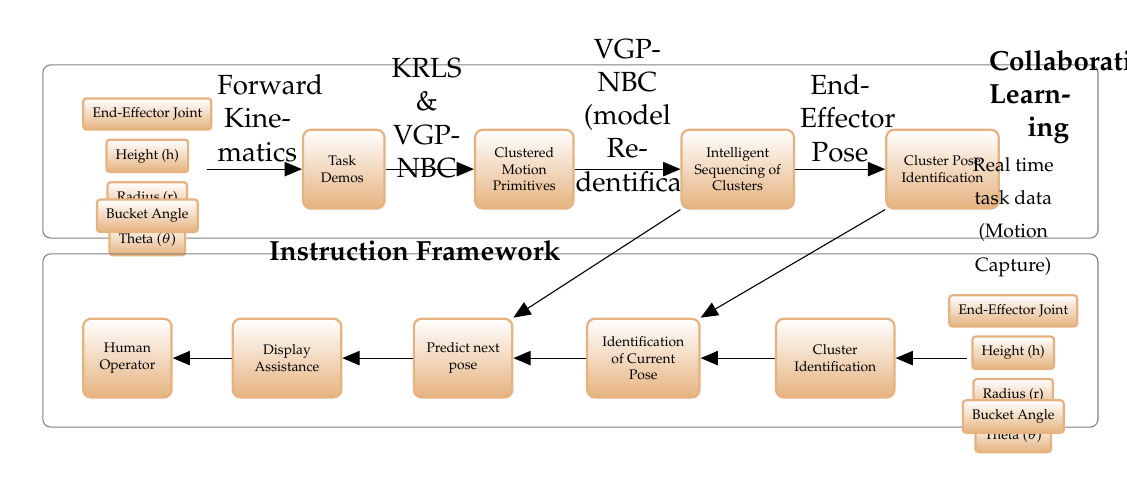
\begin{tikzpicture}[
		node distance=7mm,
		title/.style={font=\fontsize{6}{6}\color{black!50}\ttfamily},
		typetag/.style={rectangle, minimum size=2mm, rounded corners=0.4mm, thick, draw=orange!80!black!50, top color=white, bottom color=orange!80!black!50, font=\tiny},
		typetag1/.style={rectangle, minimum size=10mm, rounded corners=1mm, thick, draw=orange!80!black!50, top color=white, bottom color=orange!80!black!50, font=\tiny}
		]
		
		\node (decomp) [title, xshift=-2mm] {  };
		\node (decompd) [title, xshift=0mm] {  };
		\draw [draw=black!50,rounded corners=1mm] (decompd.north west) rectangle +(13.4cm, -2.2cm);
		
		
		
		
		\node (di) [typetag, right=of decomp.west, yshift=-5mm] { \tiny End-Effector Joint };
		\node (did) [above=of di, yshift=-5mm] { };
		%\node (didT) [above=of di, xshift=30mm, yshift=-4.5mm] { Sec 3.1 };
		\node (did1) [above=of di, xshift=75mm, yshift=-5mm] {  };
		%\node (didt2) [above=of di, xshift=87mm, yshift=-4.7mm] { Sec 3.1, 3.2 };
		\node (did2) [above=of di, xshift=102mm, yshift=-5mm] {  };
		\node (di1) [typetag, below=of di, xshift=0mm, yshift=6mm] {\tiny Height (h) };
		\node (di1d) [ below=of di.south, anchor=south, xshift=8mm, yshift=-0.2mm] { };
		\node (di2) [typetag, below=of di1.south,  xshift=0mm, yshift=6mm] {\tiny Radius (r) };
		\node (di3) [typetag, below=of di2.south, xshift=0mm, yshift=6mm] {\tiny Theta ($ \theta $) };
		\node (di4) [typetag, below=of di.south, anchor=south, xshift=0mm, yshift=-6mm] {\tiny Bucket Angle };
		\node (di5) at (2.6cm, -0.55cm) {\begin{minipage}{.4in}
			\centering
			Forward Kinematics
			\end{minipage}  };
		\node (di6) at (4.75cm, -0.55cm) {\begin{minipage}{.4in}
			\centering
			KRLS \& VGP-NBC
			\end{minipage}  };
		\node (di7) at (7.3cm, -0.55cm) {\begin{minipage}{.6in}
			\centering
			VGP-NBC (model Re-identification)
			\end{minipage}  };
		\node (di8) at (10cm, -0.55cm) {\begin{minipage}{.4in}
			\centering
			End-Effector Pose
			\end{minipage}  };
		\node (di9) at (12.4cm, -2mm) {\begin{minipage}{.4in}
			\flushright
			\textbf{Collaborative Learning}
			\end{minipage}  };
		
		\node (task) [typetag1, below=of di.east, anchor=east, text width=0.8cm, xshift=22mm, yshift=0mm] {
			\begin{minipage}{.3in}
			\centering
			Task Demos
			\end{minipage}  };
		\node (taskd) [below=of task.north, anchor=north, text width=0.8cm, xshift=-2mm, yshift=5mm] {};
		\node (taskd1) [left=of task.west, xshift=-5mm ] {};
		
		
		\node (cluster) [typetag1, below=of di.east, anchor=east, xshift=46mm, yshift=0mm]  {
			\begin{minipage}{.4in}
			\centering
			Clustered Motion Primitives
			\end{minipage}  };
		
		\node (seq) [typetag1, below=of di.east, anchor=east, xshift=74mm, yshift=0mm]  {
			\begin{minipage}{.47in}
			\centering
			Intelligent Sequencing of Clusters
			\end{minipage}  };
		
		\node (pose) [typetag1, below=of di.east, anchor=east, xshift=100mm, yshift=0mm]  {
			\begin{minipage}{.47in}
			\centering
			Cluster Pose Identification
			\end{minipage}  };
		
		
		
		\draw[->,>=triangle 45] (taskd1.east)--(task.west);
		\draw[->,>=triangle 45] (task.east)--(cluster.west);
		\draw[->,>=triangle 45] (cluster.east)--(seq.west);
		\draw[->,>=triangle 45] (seq.east)--(pose.west);
		%\draw[<->] (did.east)--(did1.west);
		%\draw[<->] (did1.east)--(did2.west);
		
		\node (di4d) [ below=of decomp.south, anchor=south, xshift=2mm, yshift=-17mm] { };
		\draw [draw=black!50,rounded corners=1mm] (di4d.north west) rectangle +(13.4cm, -2.2cm);
		
		\node (di22) at (12.2cm, -3cm) [typetag] { \tiny End-Effector Joint };
		\node (di22d) [below=of di22.south, xshift=-6mm, yshift=3.0mm] { };
		\node (di221) [typetag, below=of di22.south, xshift=0mm, yshift=6mm] {\tiny Height (h) };
		\node (di221d) [ below=of di22.south, anchor=south, xshift=8mm, yshift=-0.12mm] { };
		\node (di222) [typetag, below=of di221.south,  xshift=0mm, yshift=6mm] {\tiny Radius (r) };
		\node (di223) [typetag, below=of di222.south, xshift=0mm, yshift=6mm] {\tiny Theta ($ \theta $) };
		\node (di224) [typetag, below=of di22.south, anchor=south, xshift=0mm, yshift=-6.5mm] {\tiny Bucket Angle };
		\node (di224d) [left=of di224, xshift=0mm, yshift=0.5mm] { };
		\node (di225d) [left=of di224, xshift=-33mm, yshift=0.5mm] { };
		%\node (di225dt) [left=of di224, xshift=-12mm, yshift=-1mm] {Sec 4.1 };
		\node (di226d) [left=of di224, xshift=-56mm, yshift=0.5mm] { };
		\node (di227d) [left=of di224, xshift=-98mm, yshift=0.5mm] { };
		%\node (di225dtt) [left=of di224, xshift=-72mm, yshift=-1mm] {Sec 4.2 };
		
		\node (di10) [above=of di22, yshift=-6mm] {\begin{minipage}{.5in}
			\centering
			{\scalefont{0.7} Real time task data (Motion Capture)}
			\end{minipage}  };
		
		\node (di11) [above=of di22, xshift= -76mm, yshift=-4mm] {\begin{minipage}{2in}
			\centering
			\textbf{Instruction Framework}
			\end{minipage}  };
		
		\node[typetag1, below=of di22.west, anchor=west, xshift=-22mm, yshift=1mm] (iden) {
			\begin{minipage}{.5in}
			\centering
			Cluster Identification
			\end{minipage}  };
		\node (ident) [right=of iden, xshift=2mm] {};
		
		\node (curr) [typetag1, below=of di22.west, anchor=west, xshift=-46mm, yshift=1mm]  {
			\begin{minipage}{.47in}
			\centering
			Identification of Current Pose
			\end{minipage}  };
		
		\node (pose2) [typetag1, below=of di22.west, anchor=west, xshift=-68mm, yshift=1mm]  {
			\begin{minipage}{.4in}
			\centering
			Predict next pose
			\end{minipage}  };
		
		\node (op) [typetag1, below=of di22.west, anchor=west, xshift=-91mm, yshift=1mm]  {
			\begin{minipage}{.45in}
			\centering
			Display Assistance
			\end{minipage}  };
		
		\node (hum) [typetag1, below=of di22.west, anchor=west, xshift=-110mm, yshift=1mm]  {
			\begin{minipage}{.35in}
			\centering
			Human Operator
			\end{minipage}  };
		
		\draw[->,>=triangle 45] (ident.west)--(iden.east);
		\draw[->,>=triangle 45] (iden.west)--(curr.east);
		\draw[->,>=triangle 45] (curr.west)--(pose2.east);
		\draw[->,>=triangle 45] (pose2.west)--(op.east);
		\draw[->,>=triangle 45] (op.west)--(hum.east);
		\draw[->,>=triangle 45] (pose.south west)--(curr.north east);
		\draw[->,>=triangle 45] (seq.south west)--(pose2.north east);
		%\draw[<->] (di224d.west)--(di225d.east);
		%\draw[<->] (di226d.west)--(di227d.east);
		
		
		%\node (dep) at (3cm, 0) [title] { Dependency };
		%\draw [draw=black!50] (dep.north west) rectangle ($(dep.north east) - (0, 2cm)$);
		
		\end{tikzpicture}
	}  
}
%\pgfdeclareimage[width = 2.2 cm]{model1a}{./figures/model1-actual}
%\pgfdeclareimage[width = 2.2 cm]{model1e}{./figures/model1-estimated}
%\pgfdeclareimage[width = 2.2 cm]{model2a}{./figures/model2-actual}
%\pgfdeclareimage[width = 2.2 cm]{model2e}{./figures/model2-estimated}
%\pgfdeclareimage[width = 2.2 cm]{model3a}{./figures/model3-actual}
%\pgfdeclareimage[width = 2.2 cm]{model3e}{./figures/model3-estimated}
%\pgfdeclareimage[width = 2.2 cm]{model4a}{./figures/model4-actual}
%\pgfdeclareimage[width = 2.2 cm]{model4e}{./figures/model4-estimated}
%
%
%
%
%
%\pgfdeclareimage[width = 2.5 cm]{gpcrew}{./figures/Total-rewards-clustering}
%\pgfdeclareimage[width = 2.5 cm]{gprrew}{./figures/Total-rewards-GPR}
%\pgfdeclareimage[width = 2.0 cm]{m1e}{./figures/model1-error}
%\pgfdeclareimage[width = 2.0 cm]{m2e}{./figures/model2-error}
%\pgfdeclareimage[width = 2.0 cm]{m3e}{./figures/model3-error}
%\pgfdeclareimage[width = 2.0 cm]{m4e}{./figures/model4-error}

%\begin{minipage}{.15\textwidth}
%\centering
%\pgfuseimage{m1e} 
%\captionof{figure}{Model 1 Rewards}
%\end{minipage} \hspace{0.3em} 
%\begin{minipage}{.15\textwidth}
%\centering
%\pgfuseimage{m2e} %
%\captionof{figure}{Model 2 Rewards}
%\end{minipage}
%\begin{minipage}{.15\textwidth}
%\centering
%\pgfuseimage{m3e} %
%\captionof{figure}{Model 3 Rewards}
%\end{minipage} \hspace{0.3em} %
%\begin{minipage}{.15\textwidth}
%\centering
%\pgfuseimage{m4e} %
%\captionof{figure}{Model 4 Rewards}
%\end{minipage}

\headerbox{Construction Co-robots}{name=construction,column=0,span=1,below=objectives}{
  
  \pgfdeclareimage[width = 1.7 cm]{cat}{./figures/cat_loading2}
  
  \pgfputat{\pgfxy(5.42,-1.1)}{\pgfbox[left,base]{\pgfuseimage{cat}}}
    \begin{minipage}{0.75\textwidth}
    \begin{itemize}
    \item Robots that work with humans
   \end{itemize}
  \end{minipage}
 
  
%  \vspace{1em}
%  \begin{minipage}{0.9\textwidth}
    \begin{itemize}
    \item Complete automation impossible: safety critical decisions require human presence
    \item
      Human-robot collaborative learning and task execution
    \item
      Co-robots can train novice operators allowing experts to remain in field
    \end{itemize}
%  \end{minipage}
  
  
  
  
  
  %\begin{minipage}{.45\textwidth}
  %	\centering
  %	\pgfuseimage{cat} 
  %	%\captionof{figure}{Model 1 Rewards}
  %\end{minipage}\hspace{2.5em} 
  
}

%\begin{minipage}{.2\textwidth}
%\centering
%\pgfuseimage{var1} %
%%\captionof{figure}{Model 2 Rewards}
%\end{minipage}\hspace{2.5em}
%%\begin{minipage}{.2\textwidth}
%%\centering
%%\pgfuseimage{var2} %
%%\captionof{figure}{Model 3 Rewards}
%%\end{minipage}\hspace{5em} %
%\begin{minipage}{.2\textwidth}
%\centering
%\pgfuseimage{var3} %
%%\captionof{figure}{Model 4 Rewards}
%\end{minipage}


\headerbox{Algorithm}{name=algorithm,column=0,below=construction}{ 
  \pgfdeclareimage[height=7.5cm, width = 6.5 cm]{algo}{./figures/algo2}
  \pgfuseimage{algo}
  %\begin{minipage}[t]{\textwidth}
  %	\begin{algorithm}
  %		\DontPrintSemicolon % Some LaTeX compilers require you to use \dontprintsemicolon instead
  %		\KwIn{A finite set $A=\{a_1, a_2, \ldots, a_n\}$ of integers}
  %		\KwOut{The largest element in the set}
  %		$max \gets a_1$\;
  %		\For{$i \gets 2$ \textbf{to} $n$} {
  %			\If{$a_i > max$} {
  %				$max \gets a_i$\;
  %			}
  %		}
  %		\Return{$max$}\;
  %		\caption{{\sc Max} finds the maximum number}
  %		\label{algo:max}
  %	\end{algorithm}
  %\end{minipage}
  
}

\headerbox{Contributions}{name=contributions,column=0,below=algorithm}{
%  \vspace{0.5em}
  \begin{itemize}
%    \setlength{\itemsep}{10pt}
  \item New scalable nonparametric task models and learning algorithms
    \begin{itemize}
      \item Computationally efficient Vector-valued Gaussian Process
        Non-Bayesian Clustering (VGP-NBC)
    \end{itemize}
  \item Automatic subgoal decomposition and real-time adaptive
    controllers for executing motions generated by human operators
  \item Expertise elicitation, characterization and skill transfer
    interface design
    \begin{itemize}
      \item Semantically motivated instructional framework
    \end{itemize}
  \item Corroboration of algorithms through simulation and hardware
    experimentation

%  \item A computationally efficient Vector-valued Gaussian Processes Non-Bayesian Clustering (VGP-NBC) algorithm for real time clustering of vector-valued motion primitives.
%  \item
%    A semantically motivated instructional framework to train or assist novice users of construction co-robots that allows the co-robot to transfer learned skills from experts to novice human operators.
  \end{itemize} 
}


\headerbox{Methodology and Results }{name=methodology,column=1,span=2,below=overview}{
  \begin{multicols}{2}
    	\begin{minipage}{.47\textwidth}
		
      \textbf{Step 1: Vector-valued Gaussian Process and Non-Bayesian Clustering (VGP-NBC)} 
      \begin{itemize}
      \item
        VGP model: Actuator positions were observed; end-effector joint position ($h,r,\theta$) and bucket angle were inputs

        \pgfdeclareimage[height= 2.2 cm, width = 2.5 cm]{skel}{./figures/excavator_skeleton}
        \pgfdeclareimage[height= 2.2 cm, width = 2.5 cm]{vicon}{./figures/vicon_reduced}
        \pgfdeclareimage[width = 2.0 cm]{parrot}{./figures/ParrotDrone}
        \pgfdeclareimage[height= 1.8 cm, width = 3 cm]{cli}{./figures/clusterinput}
        \pgfdeclareimage[height= 1.8 cm, width = 3 cm]{clo}{./figures/clusteroutput}
        \pgfdeclareimage[height= 1.8 cm, width = 2.2 cm]{cl1}{./figures/clusterplot1}
        \pgfdeclareimage[height= 1.8 cm, width = 2.2 cm]{cl2}{./figures/clusterplot2}
        \pgfdeclareimage[height= 1.8 cm, width = 2.2 cm]{cl3}{./figures/clusterplot3}
        \pgfdeclareimage[height= 1.8 cm, width = 2.5 cm]{pose}{./figures/pose}
        \pgfdeclareimage[height= 1.8 cm, width = 2.5 cm]{111}{./figures/1}
        \pgfdeclareimage[height= 1.8 cm, width = 2.5 cm]{222}{./figures/2}
        
        \vspace{1em}
        
        
        \begin{minipage}{0.35\textwidth}
	  \centering
	  \pgfuseimage{vicon} 
          %	\captionof{figure}{Set Up}
        \end{minipage}\hspace{2.5em} 
        \begin{minipage}{0.35\textwidth}
	  \centering
	  \pgfuseimage{skel} %
          %	\captionof{figure}{Excavator Skeleton}
          %	{\small Excavator Skeleton}
        \end{minipage}\vspace{1em}
        
        %{\textbf{Figure:} Experimental setup and Excavator Skeleton}
        %\pgfuseimage{vicon}\hspace{1em} 
        \captionof{figure}{Experimental setup and excavator skeleton}
        %\pgfuseimage{skel}\hspace{1em} 
        %\captionof{figure}{ i) Set Up, ii) Excavator Skeleton}	
      \end{itemize}
      \begin{itemize}
      \item Motion primitives such as \textsc{boom-raise} or
        \textsc{bucket-curl} arise from different VGP models.
      \item
        Non-Bayesian Clustering \cite{Grande14_TNN}: Hypothesis test used to determine and cluster different VGP models (Figure \ref{seg}).
        \begin{equation}\label{lrt}
          \frac{P(y \mid M_i)}{P(y \mid M_j)} \begin{array}{c} \hat M_i \\ \gtreqless \\ \hat M_j \end{array}\eta
        \end{equation}
      \item
        Changepoints for the clusters match actual end-effector poses which a human trainer might utilize to train novice operators. 
      \end{itemize}
      
    \end{minipage}
    \begin{minipage}{.23\textwidth}
      \centering
      \pgfuseimage{cli} 
    \end{minipage}
    \begin{minipage}{.23\textwidth}
      \centering
      \pgfuseimage{clo} %
    \end{minipage}
    \captionof{figure}{Cluster segments identified by the algorithm for a truck loading task}\label{seg}
    \begin{itemize}
    \item
      Algorithm yields similar clusters for data with different temporal properties (Figure \ref{cluster}). 
    \end{itemize}
    \begin{minipage}{.15\textwidth}
      \centering
      \pgfuseimage{cl1} 
      %	\captionof{figure}{Cluster Input}
    \end{minipage}
    \begin{minipage}{.15\textwidth}
      \centering
      \pgfuseimage{cl2} %
      %	\captionof{figure}{Cluster Output}
    \end{minipage}
    \begin{minipage}{.15\textwidth}
      \centering
      \pgfuseimage{cl3} %
      %	\captionof{figure}{Cluster Output}
    \end{minipage}
    \captionof{figure}{Segmentation with different temporal characteristics}\label{cluster}
    \textbf{Step 2: Instruction Framework}
    \begin{itemize}
    \item
      On-line re-identification of clusters, coupled with learned sequence of clusters.
    \item
      Automated Flash-card instructions to guide a novice operator, learning a task.
    \end{itemize}
    
    \begin{minipage}{.15\textwidth}
      \centering
      \pgfuseimage{111} 
      %	\captionof{figure}{Cluster Input}
    \end{minipage}
    \begin{minipage}{.15\textwidth}
      \centering
      \pgfuseimage{pose} %
      %	\captionof{figure}{Cluster Output}
    \end{minipage}
    \begin{minipage}{.15\textwidth}
      \centering
      \pgfuseimage{222} %
      %	\captionof{figure}{Cluster Output}
    \end{minipage}
    \captionof{figure}{Flash cards and cluster poses}
    
  \end{multicols}
}

%\headerbox{Non Stationary MDP}{name=nsmdp,column=2,below=results,above=bottom}{ 
%\begin{itemize}
%\item Non Stationary MDP's characterized by tuple $<S,A,T,R>$ where reward r is dynamic,i.e $r = r(t)$
%\item Deisenroth et al.\cite{Dei08} details work on model-based Reinforcement learning using Gaussian Processes, describing flexibility of GP and using predictive variance for exploration 
%\item Non Stationary MDPs solve  for $\pi^*$ by using tuple $<S,A,T,\hat{r}>$, where $\hat{r}$ is estimated using a GP BNP
%\end{itemize}
%
%}

\headerbox{Guided vs Unguided}{name=demos,column=1,below=methodology}{ 
	
  \pgfdeclareimage[height= 2.5 cm, width = 3.5 cm]{box}{./figures/boxplot}
  %\pgfdeclareimage[height= 2.5 cm, width = 3.5 cm]{boxa}{./figures/box_actions}
  \pgfdeclareimage[height= 2.5 cm, width = 3.0 cm]{iti}{./figures/iterative}
  
	\begin{itemize}
	\item Comparison for truck loading task: Better performance in guided mode
          %		\item The task was performed more efficiently in the ``guided'' mode.
	\end{itemize}
	\vspace{-1.5em}
        %	\begin{minipage}{.15\textwidth}
	\centering
	\pgfuseimage{box} 
	%	\captionof{figure}{Cluster Input}
        %	\end{minipage}
        %	\begin{minipage}{.15\textwidth}
	%\centering
	%\pgfuseimage{boxa} %
	\begin{minipage}{0.9\textwidth}
	  \captionof{figure}{Completion time for the two modes}\label{comp}
	\end{minipage}
	
	\vspace{-1em}
	\begin{minipage}{.60\textwidth}
	  \begin{itemize}
	  \item Performance comparison between first and second cycle.
	    
	  \end{itemize}
	  
	\end{minipage}		
        %	\end{minipage}
	\begin{minipage}{.35\textwidth}
	  
	  \pgfuseimage{iti} %
	\end{minipage}
	
        %		\begin{minipage}{0.9\textwidth}
        %			\captionof{figure}{Performance compared over 2 cycles}
        %				\end{minipage}
        %	\end{minipage}
	
        
        
}

\headerbox{References}{name=references,column=2,below=methodology}{
  
  \renewcommand{\section}[2]{\vskip 0.05em} 
  \nocite{*} 
  \small{
    \bibliographystyle{unsrt}
    \bibliography{bib} 
    
  }
}


\end{poster}

\end{document}
